% latex - beamer presentation

\documentclass[pdf,hideothersubsections]{beamer}
\usepackage{beamerthemeshadow}
\mode<presentation>
  {
    \usefonttheme{structuresmallcapsserif}
    \usetheme{PaloAlto}
    \usecolortheme{seagull}
    %\useinnertheme{circles}
%    \useoutertheme{tree}
  }

\usepackage{xmpmulti}


\usepackage{hyperref}
\hypersetup{
    pdffitwindow=true,     % window fit to page when opened
    colorlinks=true,       % false: boxed links; true: colored links
    linkcolor=orange,          % color of internal links (change box color with linkbordercolor)
    citecolor=green,        % color of links to bibliography
    filecolor=magenta,      % color of file links
    urlcolor=blue           % color of external links
}



% Fonts/encoding
\renewcommand{\UrlFont}{\scriptsize}
\usepackage[utf8]{inputenc}
\usepackage[T1]{fontenc}
%\usepackage[sc,medium,raggedright]{titlesec}
\usepackage{newtxmath}
%\usepackage{libertine}
\usepackage[osf]{ebgaramond}

\graphicspath{{Figures/}}

\begin{document}
\title{Periodic Motion}  
\author{Caltech: ph2a}
\date{26 - Sep - 2017}
%\logo{
\includegraphics[height=0.5cm]{../caltech_logo.png}}

\frame{\titlepage} 

\frame{\frametitle{Table of contents}\tableofcontents} 


\section{Class Overview}
\frame{\frametitle{Overview}
\begin{enumerate}
\item All info on class website\footnotemark 
\item Lectures are Tuesday and Thursday
\item try out different sections; problems solving is key!
\item Use piazza for group chat / anon discussions, feedback
\item HWK due every Wed. Quizzes every other Tuesday. Final in Dec.

\end{enumerate}

\footnotetext[1]{\url{https://piazza.com/caltech/fall2017/ph2a}}
}


\section{Simple Harmonic Oscillator}
\frame{\frametitle{The Simple Harmonic Oscillator}
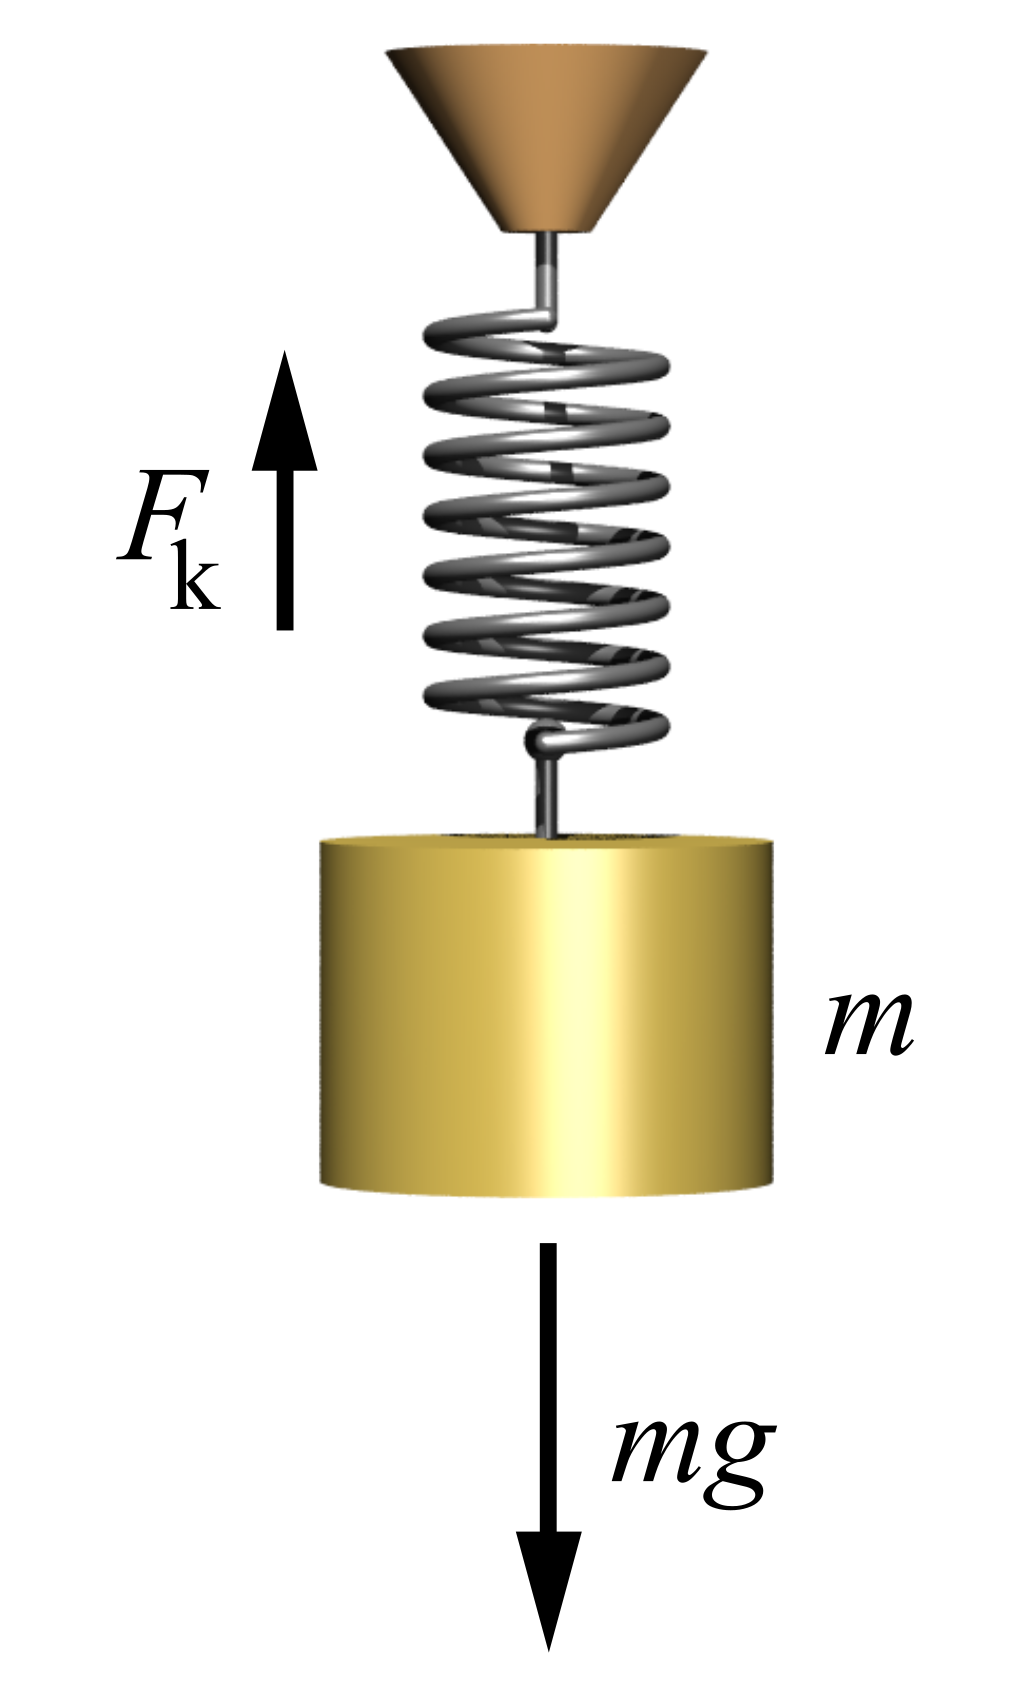
\includegraphics[height=3cm]{Mass-spring-system.png}

\begin{itemize}
\item Covered in ph1a (mass-spring, pendulums) \pause
\item Covered in ph1b/c (RLC Circuits) \pause
\item Extremely useful in engineering / sciences \pause
\item ``Just'' the study of 2$^{nd}$ order differential equations
\end{itemize}

}

\subsection{Demo: Ball on Spring}
\begin{frame}
\frametitle{Interactive Demo}
\centering
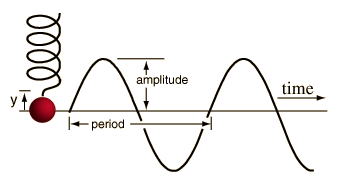
\includegraphics[height=3cm]{2015416-94550395-2754-sshm.png}
\begin{itemize}
\item \url{https://phet.colorado.edu/en/simulation/mass-spring-lab}
\item \url{http://demonstrations.wolfram.com/DrivenDampedOscillator/}
\item \url{http://demonstrations.wolfram.com/SimpleHarmonicMotionForASpring/}
\end{itemize}
\end{frame}


\subsection{General Solution}
\frame{\frametitle{Harmonic Oscillator Equations}
\centering
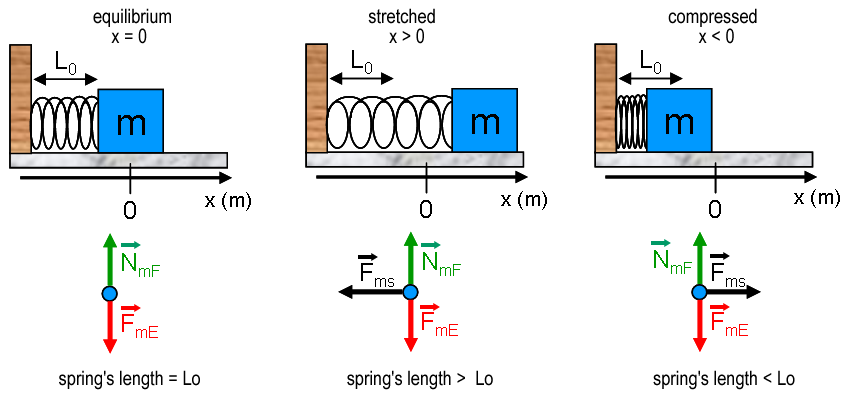
\includegraphics[height = 4cm]{Hookeslawb.png} \\ \pause
\begin{align*}
  \onslide<1->{F &= m \frac{d^2x}{dt^2} \\}
  \onslide<2->{- k x &= m \ddot{x}}
\end{align*}
}

\frame{\frametitle{Solution I:}
The Diff Eq we want to solve (for x(t)): $- k x = m \ddot{x}$
\pause
\begin{align*}
  \onslide<2->{x(t) &= A cos(\omega t) + B sin(\omega t) \\}
  \onslide<3->{\frac{dx}{dt} &= -\omega A sin(\omega t) + \omega B cos(\omega t) \\}
  \onslide<4->{\frac{d^2x}{dt^2} &= -\omega^2 \left[A cos(\omega t) + B sin(\omega t)\right] \\}
                    \onslide<5->{&= -\omega^2 x(t)}
\end{align*}

\onslide<5->{Therefore, $\omega = \sqrt{k/m}$. Define $\omega_0 \equiv \sqrt{k/m}$}

}

\frame{\frametitle{Solution II:}
Use a phase shift in the cosine instead of sine and cosine:
\pause
\begin{align*}
  \onslide<2->{x(t) &= D~cos(\omega t + \phi_0) \\}
  \onslide<3->{\frac{dx}{dt} &= -\omega D sin(\omega t + \phi_0) \\}
  \onslide<4->{\frac{d^2x}{dt^2} &= -\omega^2 D cos(\omega t + \phi_0) \\}
                 \onslide<4->{&= -\omega^2 x(t)}
\end{align*}
}

\frame{\frametitle{Boundary Conditions}
In both cases, there are two free constants (A \& B, or D \& $\phi_0$). \\
\pause
These constants are set to force the solution to match any 'Boundary' conditions: \pause
\begin{itemize}
\item initial displacement \pause
\item initial velocity \pause
\item e.g., mass is released at t=0 with x = x$_0$
\end{itemize}

}

\subsection{Damping / Friction}
\frame{\frametitle{SHO + Damping}
What about adding some frictional damping?
\pause
\begin{itemize}
\item Friction = force proportional to velocity
\pause
\item Mechanical: $m \ddot{x} + b \dot{x} + k x = 0$
\pause
\item Electrical (demo): $L \ddot{Q} + R \dot{Q} + (1/C) Q = 0$
\end{itemize}
\pause

\begin{block}{Damping}
Resistance is the electrical equivalent of friction.
\end{block}

\pause
\centering
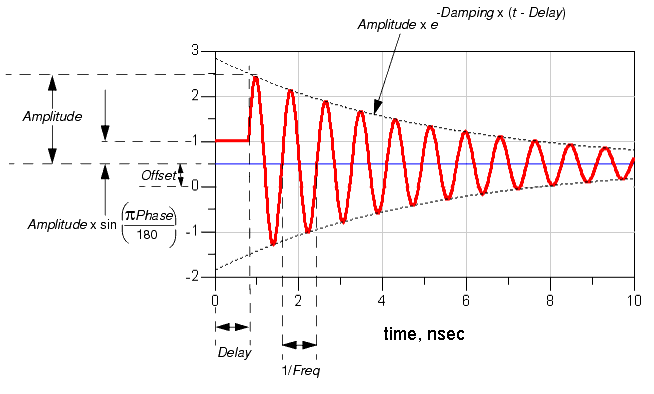
\includegraphics[width=5cm]{damped_sine.png}
}


\section{Differential Equations} 
\subsection{Types}
\frame{\frametitle{Types of Diff. Eq.}
\centering
\begin{tabular}{l|c|c|c|}
\hline
Name/Type  & \textbf{Variables} & \textbf{Order} & \textbf{Linearity} \\
\hline \pause
Ordinary & 1 & 1+ & Yes  \\
\hline \pause
Partial & 2+ & 1+ & Yes ? \\
\hline \pause
Linear & 1+ & 1+ & Yes \\
\hline \pause
Non-Linear & 1+ & 1+ & No \\
\hline
\end{tabular}
}


\frame{\frametitle{Diff Eq Examples}
\begin{block}{Harmonic Oscillator: Damped mass on spring}
a \emph{linear}, 2$^{nd}$ order, ordinary differential equation \\
$m \ddot{x} + b \dot{x} + k x = 0$
\end{block}
\pause
\begin{exampleblock}{Harmonic Oscillator: RLC Circuit}
a \emph{linear}, 2$^{nd}$ order, ordinary differential equation \\
$L \ddot{Q} + R \dot{Q} + (1/C) Q = 0$
\end{exampleblock}
\pause
\begin{alertblock}{Driven Harmonic Oscillator}
a \emph{linear}, 2$^{nd}$ order, ordinary differential equation \\
$m \ddot{x} + b \dot{x} + k x =  F_0 sin(\omega t)$
\end{alertblock}

}


\section{Harmonic Oscillator + Complex Math}
\subsection{Complex Numbers}
\frame{\frametitle{Complex Numbers}
\begin{itemize}
\item See \href{https://piazza.com/caltech/fall2017/ph2a/resources}{Handout} on complex numbers on course website.
\pause
\item Differing notations: $i = \sqrt{-1}$ or $(j = \sqrt{-1})$
\pause
\item Complex Variables: 
\end{itemize}
\pause

\begin{align*}
  \onslide<3->{\tilde{z} &= x + i y \\}
  \onslide<4->{        &= Re\left\{\tilde{z}\right\} + i\,Im\left\{\tilde{z}\right\} \\}
  \onslide<5->{\tilde{z}^{*} &= x - i y (\rm complex~conjugate)}
\end{align*}

\begin{align*}
  \onslide<6->{|\tilde{z}|^2 &= \tilde{z}^{*}\tilde{z} \\}
  \onslide<7->{              &= (x + i y)(x - i y) \\}
  \onslide<8->{              &= x^2 + y^2 }
\end{align*}
}


\subsection{Euler's Formula}
\begin{frame}
\frametitle{Euler's Formula}

\begin{block}{\href{http://mathworld.wolfram.com/EulerFormula.html}{Euler's Formula}}
$e^{i \phi} = \cos{\phi} + \mathrm{i} \sin{\phi}$
\end{block}
\pause
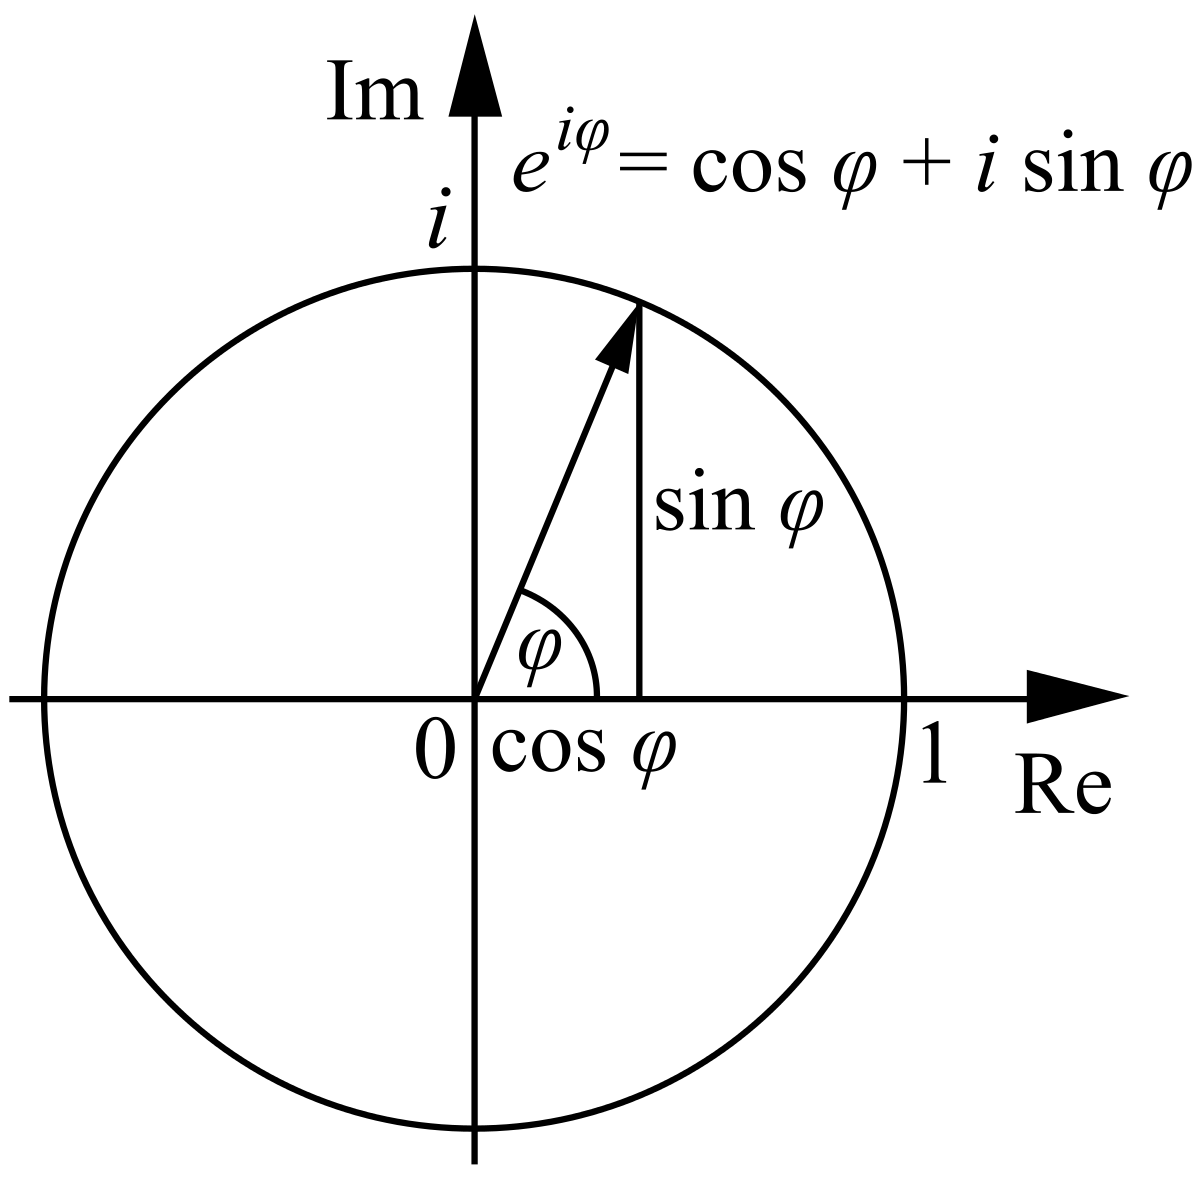
\includegraphics[width=3cm]{Euler-formula.png}
\pause
\begin{itemize}
\item $|e^{i \phi}| = 1$
\pause
\item $1 + e^{i \pi} = 0$
\end{itemize}

Mesmerizing GIF: \url{http://i.imgur.com/BI1zPwO.gif}

\end{frame}

\subsection{Complex Solutions to SHO}
\begin{frame}
\frametitle{Complex Solutions}
\begin{itemize}
\item Complex exponentials make D.E. solving much easier
\pause
\item Actual displacement is not imaginary; this is book-keeping
\pause
\end{itemize}
Guess: $\tilde{x}(t) = A e^{i (\omega t + \phi_0)}$ \\
\pause
$\ddot{x} = -(k/m) x$ \\
\pause
$\dot{x} = i \omega x$ \\
\pause
$\ddot{x} = -\omega^2 x$ \\
Plug in the guess into the differential equation:
\begin{align*}
-\omega^2 x &= (-k/m) x \\
\omega &= \sqrt{k/m} \\
x(t) &= A e^{i (\sqrt{k/m} t + \phi_0)}
\end{align*}
\pause
Taking the real part, we get: \\
\pause
$x(t) = Re\left\{\tilde{x}(t)\right\} = A cos(\omega t + \phi_o)$

\end{frame}

\section{Damped Harmonic Oscillator}
\begin{frame}
\frametitle{Complex approach to damped SHO}
Use the same approach as before:
\begin{itemize}
\item $m \ddot{x} + b \dot{x} + k x = 0$
\pause
\item $x(t) = A e^{i (\omega t + \phi_0)}$
\pause
\item $-m \omega^2 x + i \omega b x + k x = 0$
\end{itemize}
\pause
Dividing by $m$, we get a quadratic equation for $\omega$: \\
\pause
$\omega = \sqrt{\omega_0^2 - (\frac{b}{2 m})^2} + i \frac{b}{2 m}$ \\
\pause
Let's call the real part $\omega$ and plug back into the guess for x(t):
\pause
$\tilde{x} = A e^{i (\omega t + \phi_0)} e^{-(b/2 m) t}$\\
\pause
Taking the real part, we find there is an oscillatory component multiplied by a decaying exponential (the damping): \\
\pause
$Re\left\{\tilde{x}\right\} = x = A \cos(\omega t + \phi_o) e^{-(b/2 m) t}$

\end{frame}

\begin{frame}
\frametitle{Decaying Oscillation}

\centering
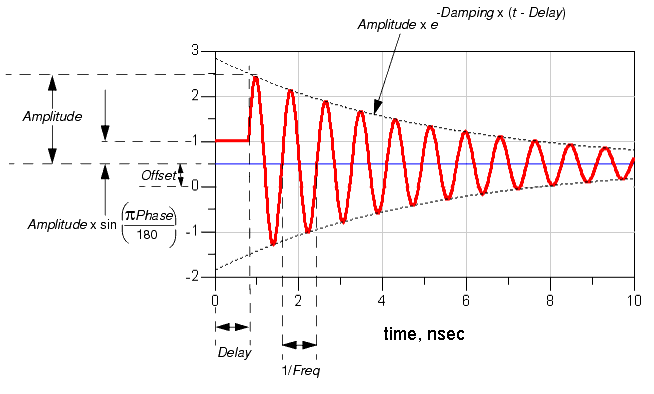
\includegraphics[width=8cm]{damped_sine.png}

\end{frame}

\section{Summary}
\begin{frame}
\frametitle{Summary}
\begin{itemize}
\item Many physical systems involving small vibrations can be represented as a Simple Harmonic Oscillator.
\pause
\item Complex exponentials can be used to solve oscillator problems.
\pause
\item Guess solutions; set constants by setting (Dirichlet, Neumann, Cauchy) boundary conditions.
\pause
\item Imaginary part of the complex frequency corresponds to damping.
\end{itemize}
\end{frame}

\end{document}

